\subsection{Второй этап. Рандомизатор и защитный интервал}
На предыдущем этапе мы получили некоторую основу для нашей модели.
Все дальнейшие изменения внесут новые элементы в последовательность преобразований, что бы приблизить ее к реальной.
Расширенная схема преобразований отображена на Рис.\ref{fg:OFDM-2}) 
\begin{figure}[h!]
\centering
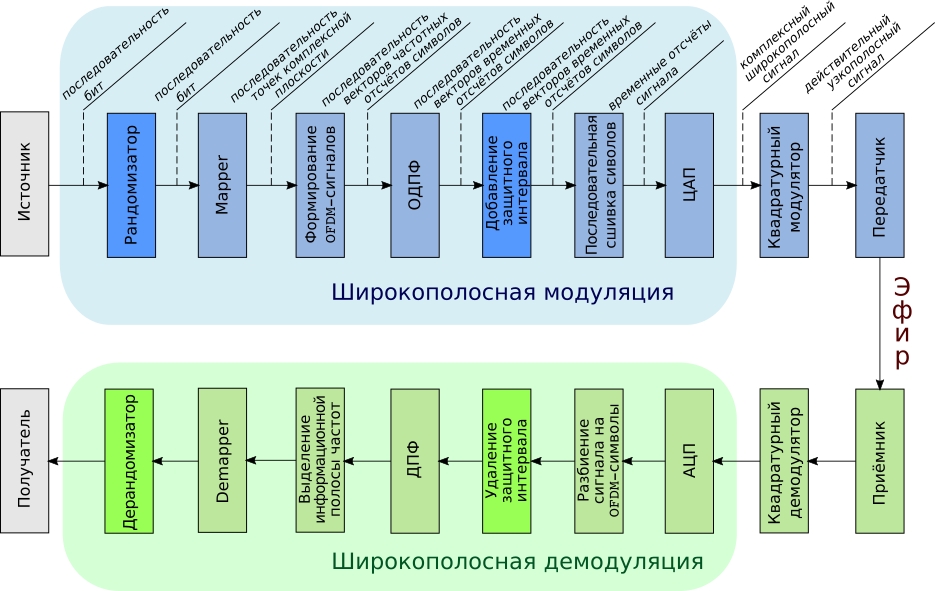
\includegraphics[width=1\textwidth]{OFDM-2}
\caption{Последовательность преобразований сигнала} \label{fg:OFDM-2}
\end{figure}

Задачей второго этапа является внедрение рандомазатора и защитного интервала. 
 Подробно роль этих компонент описана в параграфах (ссылки)
 
 Нам понадобятся еще два параметра:
 \begin{itemize}
 \item \textit{register = [100101010000000]} -   инициирующая последовательность является частью стандартов связи и считантся известной передатчику и приемнику, так что  имеем массив 15 бит в качестве параметра.
 \item \textit{t\underline{ }guard = n\underline{ }/8}- защитный интервал. 
 \end{itemize}
 
\subsubsection{Передатчик}

\subsubsection*{Рандомизатор}
Принципиальная схема устройства представлена на Рис. \ref{fg:rand}) 

\begin{figure}[h!]
\centering
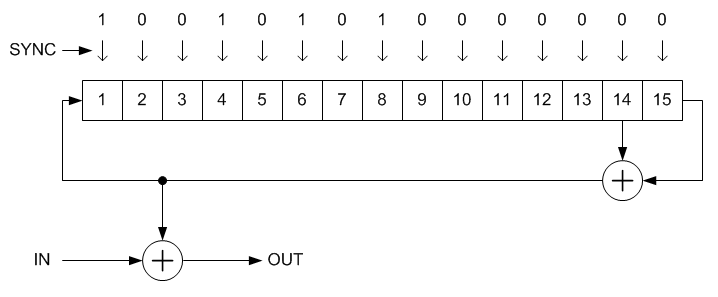
\includegraphics[width=1\textwidth]{rand}
\caption{Рандомизатор} \label{fg:rand}
\end{figure}

Функция-рандомизатор должна производить обработку сигнала в такой же последовательности. 
Регистр имеет конечную величину, моделируется либо массивом либо очередью размером 15.
После каждой операции XOR двух младших бит регистра ее результат записывается в старший бит, а все прочичие биты сдвигаются к младшему. 
Тем самым происходит генерация псевдослучайной последровательности определенного типа. 
Далее, получившийся бит, кроме того что записывается обратно в регистр, снова подвергается операции XOR, на этот раз с битом информационной последовательности. 
Последовательность бит, получившихся в результате смешения бит псевдослучайной последовательности и бит информационной последовательности отправляется на выход функции. 

Это лишь одна из возможных схем скремблирования данных. Стандарты связи предусматривают схемы для смешения не отдельных бит, а целых последовательностей, например, на более поздних этапах обработки в стандарте DVB-T производится скремблирование (перемежение) целых кадров.   
Целью таких операций является защита данных от потери. 
При такой обработке, в случае утери сигнала потеряется не последовательность информации,а отдельные ее участки, которые за частую можно восстановить с помощью помехоустойчивого кодирования. 
Кроме того, роль рандомизатора важна  для устранения/сглаживания пик-фактора (ссылка): рандомизатор "размазывает" энергию сигнала по всему спектру.

Для демонстрации этого свойства рандомизатора предлагается написать дополнительную функция, цель которой построить график мощности, а так же посчитать значение пик-фактора по соответсвующей формуле:

$ P = 20\times \log_{10}{\max{\frac{|S(t)|}{S_{ср}}}}$

Можно оценить результаты работы рандомизанара на Рис. \ref{fg:with|without}

\begin{figure}[H]
\begin{minipage}[h]{\linewidth}
\center{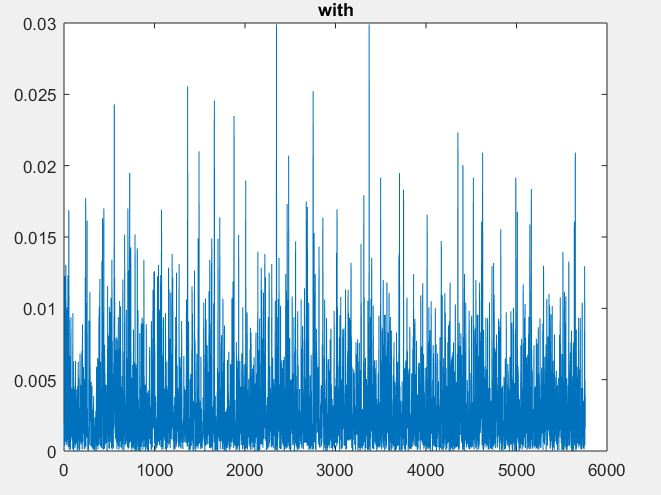
\includegraphics[width=0.5\linewidth]{with} \\ a)}
\end{minipage}

\begin{minipage}[h]{\linewidth}
\center{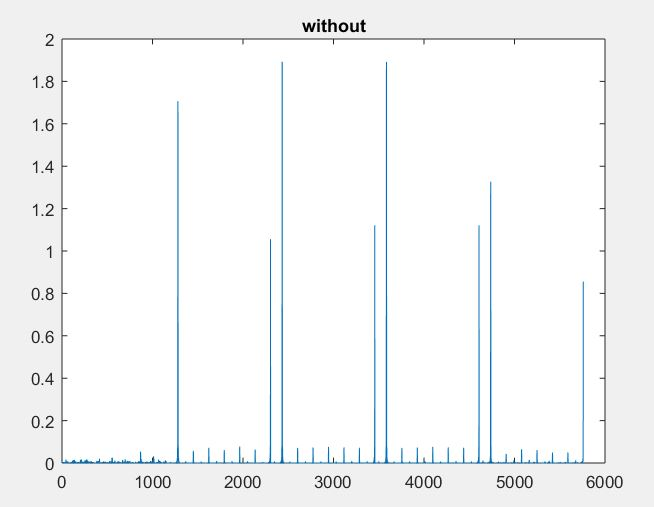
\includegraphics[width=0.5\linewidth]{without} \\ b)}
\end{minipage}
\caption{Сигнал a)с рандомизатором и пик-фактором 10.5 дБ и b)без рандомизатора и пик-фактором 32.8 дБ}
\label{fg:with|without}
\end{figure}

\subsubsection*{Защитный интервал}

Защитный интервал исполняет множество функций, но прежде всего он  вводится для предотрвращения межсимвольной интерференции и защиты от прочих наложений.
Простейший способ ввести интервал - разнести символы по времени. 
Однако такое использование канала неэффективно и затратно, поскольку требует точной синхронизации приемника и передатчика.

Рекомендуется реализовать более эффективный способ -  добавление префиксного защитного интервала.
Из названия следует, что защитный интервал добавляется спереди символа.
Однако вместо представляет собой копию  некоторого участка самого сигнала. 
Для наибольшей эффективности в качестве дублера берется окончание OFDM-символа, таким образом, сигнал становится "закольцован" - начало повторяет конец. 

Удобство такой системы станет понятно на дальнейших этапах (синхронизация). 
Пока же достаточно понимать, что при преобразовании Фурье  закольцованного сигнала  потребуются все те же \textit{n\underline{ }fft} отсчетов, т.е. конечный результат (спектральные компененты) не изменятся от переноса части символа в его начало. 

Итак, функция, добавляющая защитный интервал, возвращает последовательность отсчетов сигналов с префиксом-копией конца сигнала. ( Рис. \ref{fg:guard}) 


\begin{figure}[h!]
\centering
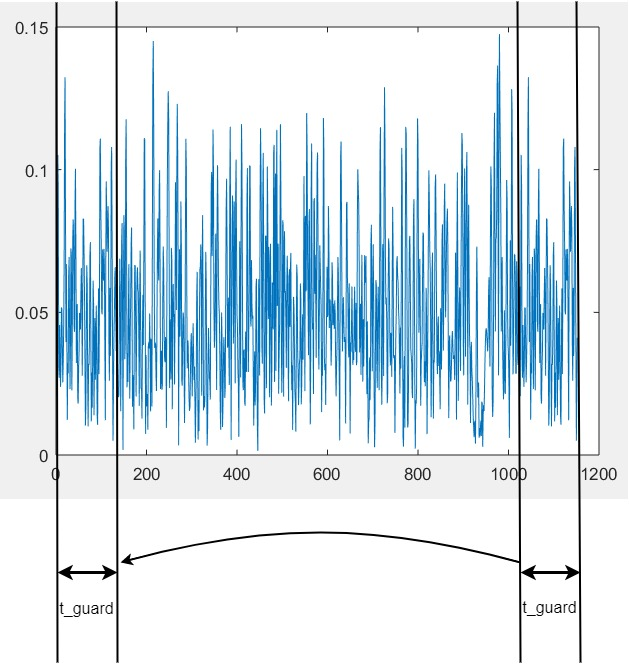
\includegraphics[width=1\textwidth]{guard}
\caption{Защитный интервал} \label{fg:guard}
\end{figure}

\subsubsection{Канал}

Канал все еще не вносит искажений, поэтому не моделируется.

\subsubsection{Приемник}

\subsubsection*{Дерандомизатор}

Для восстановления исходной последовательности требуется произвести ту же самую процедуру скремблирования, которая производилась в передатчике. 

\subsubsection*{Удаление защитного интервала}
Пока что прием сигнала не требует синхронизации, так что для удаления защитного интервала достаточно отбросить лишние с конца символа отсчеты перед перобразование Фурье.

\subsubsection {Вопросы}
Почему рандомизатор имеет такой вид и чем ценна процедура XOR для него?
Чем опасен пик-фактор?